\section{The MICE Experiment}
\label{sec:MICE}
  \subsection{Overview}
  \label{subsec:Overview}
  The Muon Ionization Cooling Experiment (MICE) will be the first practical demonstration of ionization cooling of muons. Cooling refers to a reduction in the emittance of a beam, that is, the phase space volume occupied. Beam cooling is required for any future facility based on high intensity muon beams, such as a Neutrino Factory~\cite{ISS-Physics}, the ultimate tool to study leptonic CP symmetry violation, or Muon Collider~\cite{MC_Overview}, a potential route to multi-TeV lepton - anti-lepton collisions. Muon beams are generated via pion decay, leading to a large initial phase space distribution, which must be shrunk in order for a reasonable fraction of the beam to fall within the acceptance of downstream acceleration components. Without cooling much of the muon beam is lost, leading to a severe reduction in useful particle rates.   

  The short muon lifetime requires a fast beam cooling technique which traditional cooling techniques are unable to provide.  Ionisation cooling was proposed in the early 1970s~\cite{Skrinsky, Neuffer}, but has yet to be demonstrated.  Ionization cooling reduces beam emittance by first passing a beam through some suitable, low atomic number material, such a hydrogen.  This leads to reduction in beam momentum in all directions due to ionisation energy losses.  After the absorber, momentum is restored in the longitudinal direction only by means of RF cavities.  The sequence is repeated leading to an overall reduction in the transverse phase space of the beam.

  \begin{figure}[bht]
    \begin{center}
      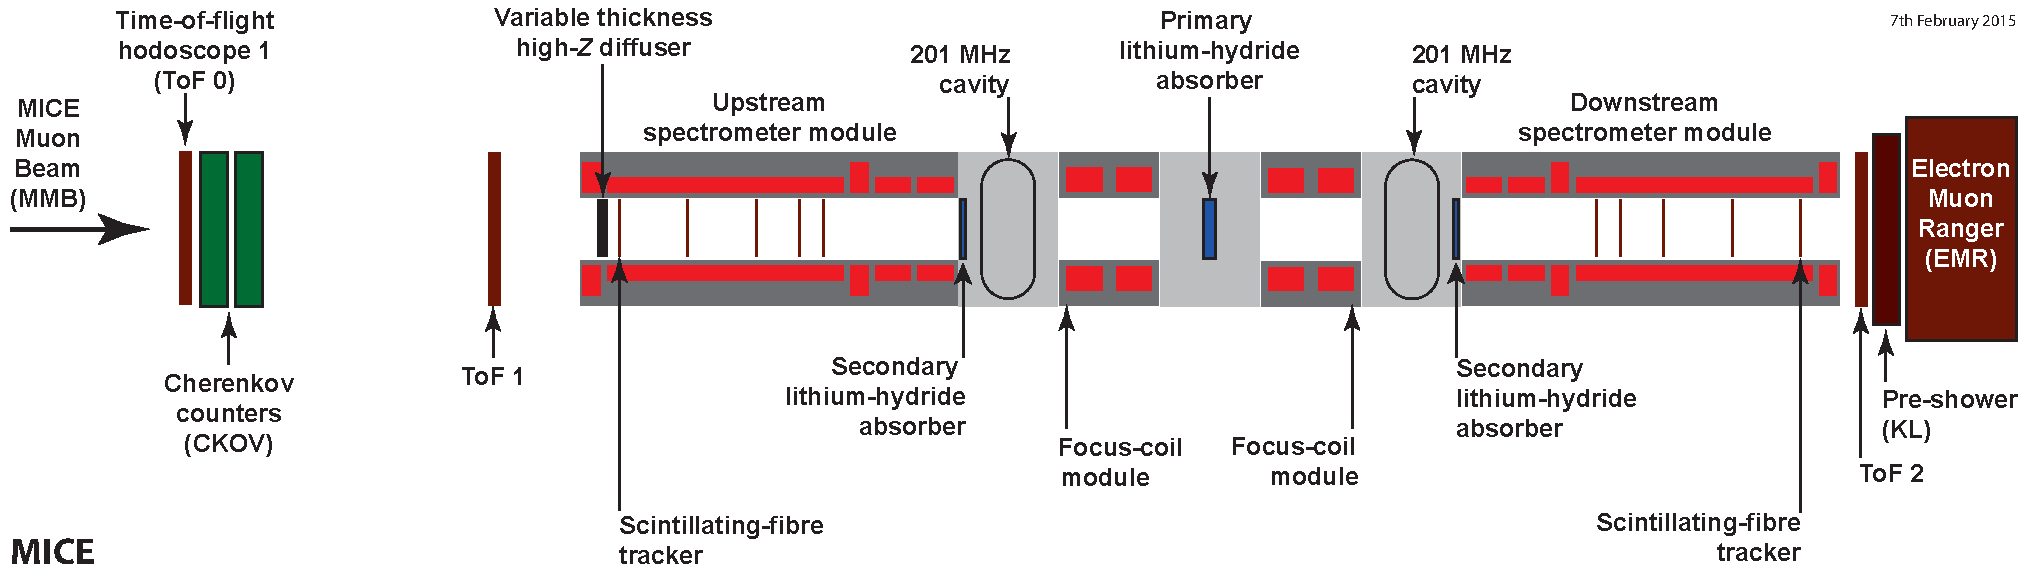
\includegraphics[width=1.0\linewidth]{01-MICE/Cooling-demo-labels.pdf}
      \caption{\label{fig:CoolingChannel} The downstream beam line and final cooling channel. The diffuser is used to increase the beam emittance prior to cooling. The primary absorber can be swapped between liquid hydrogen and solid lithium hydride.}
    \end{center}
  \end{figure}

  MICE will represent the first practical demonstration of muon cooling. A schematic of the full MICE cooling channel, including ionisation energy loss and longitudinal acceleration, is shown in figure~\ref{fig:CoolingChannel}.

  MICE is based at Rutherford Appleton Laboratory, U.K., using the ISIS synchrotron as a proton driver to generate the muon beam.  The MICE beamline is described in detail in~\cite{MiceBeamline}.  MICE recently completed Step~I of its programme, consisting of the muon beamline with particle identification (PID). The next step in the programme, Step IV, which introduced the trackers and the first absorber module, producing transverse emittance reduction, began taking data in 2015. The demonstration of sustainable cooling, which includes longitudinal re-acceleration, will begin data taking in 2018.

%   \begin{figure}[tb]
%     \begin{center}
%       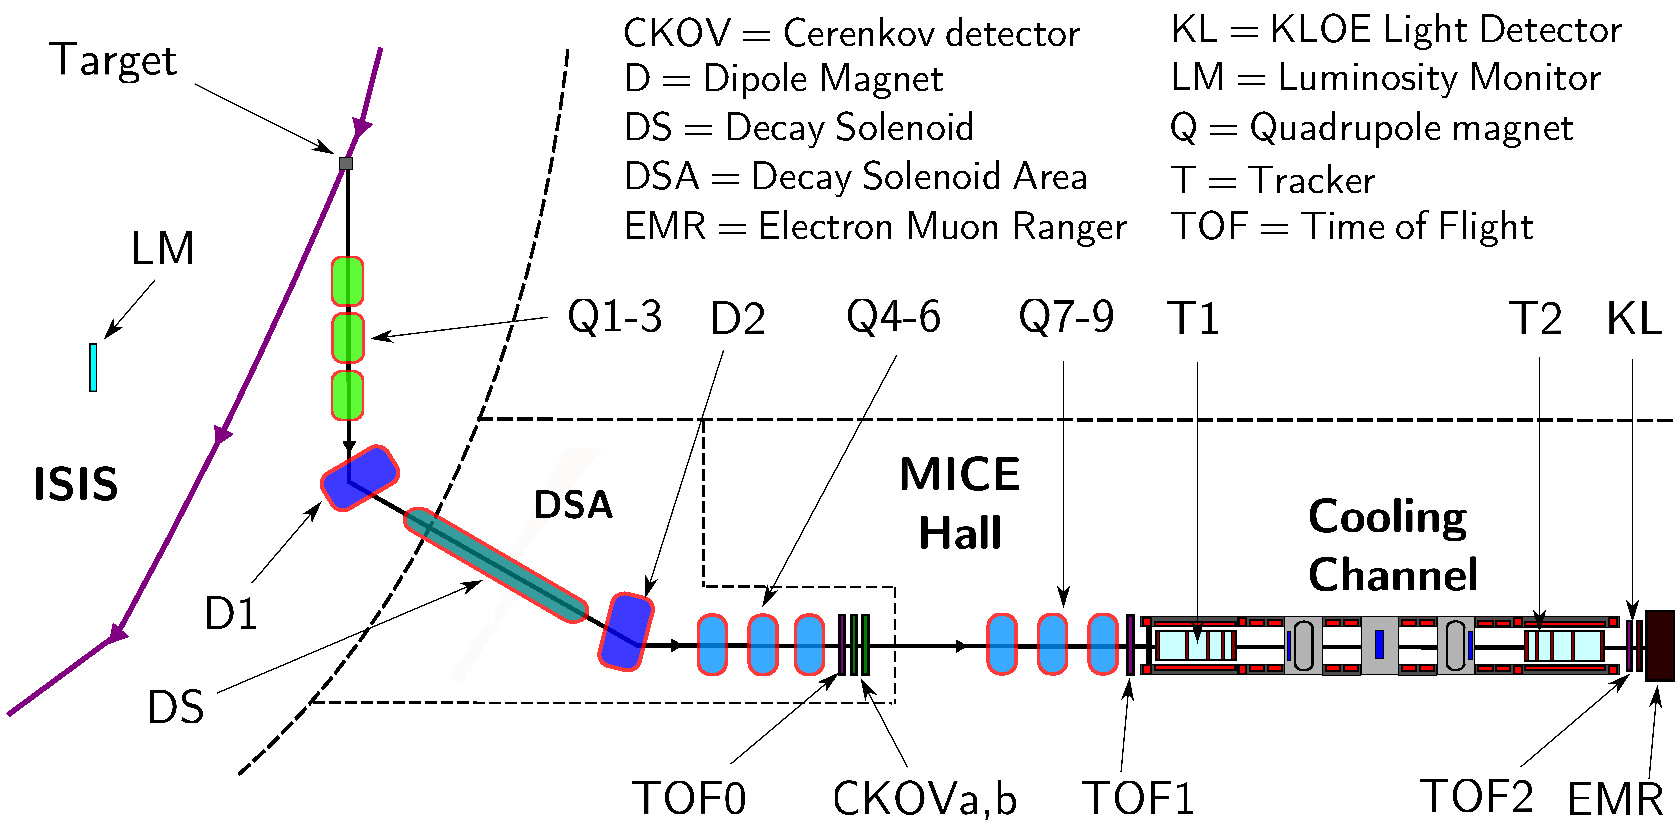
\includegraphics[width=0.75\linewidth]{01-MICE/BeamLineDEMOSans.pdf}
%       \caption{\label{fig:Beamline}The MICE Muon Beamline. A pion production target intercepts the protons of the circulating ISIS beam. Some of the subsequent pions are then captured by quadrupoles and guided down the beamline, passing through various PID detectors along the way, before delivery to the cooling channel itself. Emittance is measured immediately before and after the cooling channel using the scintillating fibre trackers.}
%       \end{center}
%   \end{figure}

  \subsection{The Scintillating Fibre Trackers}
  \label{subsec:Trackers}
  MICE is equipped with two identical, high precision scintillating fibre (``scifi'') trackers, described in~\cite{MiceTrackers}. Each tracker is housed in a superconducting solenoid that provides a uniform 4\,T field over the tracking volume. Tracker~1 is located upstream of the cooling channel, Tracker~2 downstream.  Each tracker consists of 5 detector stations, labelled 1 to 5, as illustrated in figure~\ref{fig:Trackers}. The upstream tracker, TKU, is orientated such that Station~5 sees the beam first, while the downstream tracker, TKD, is rotated by 180$^\circ$ such that Station~1 sees the beam first, thus in both trackers Station~1 is always nearest to the cooling channel (see figure~\ref{fig:CoolingChannel}).
  
  \begin{figure}[tbh]
    \centering
    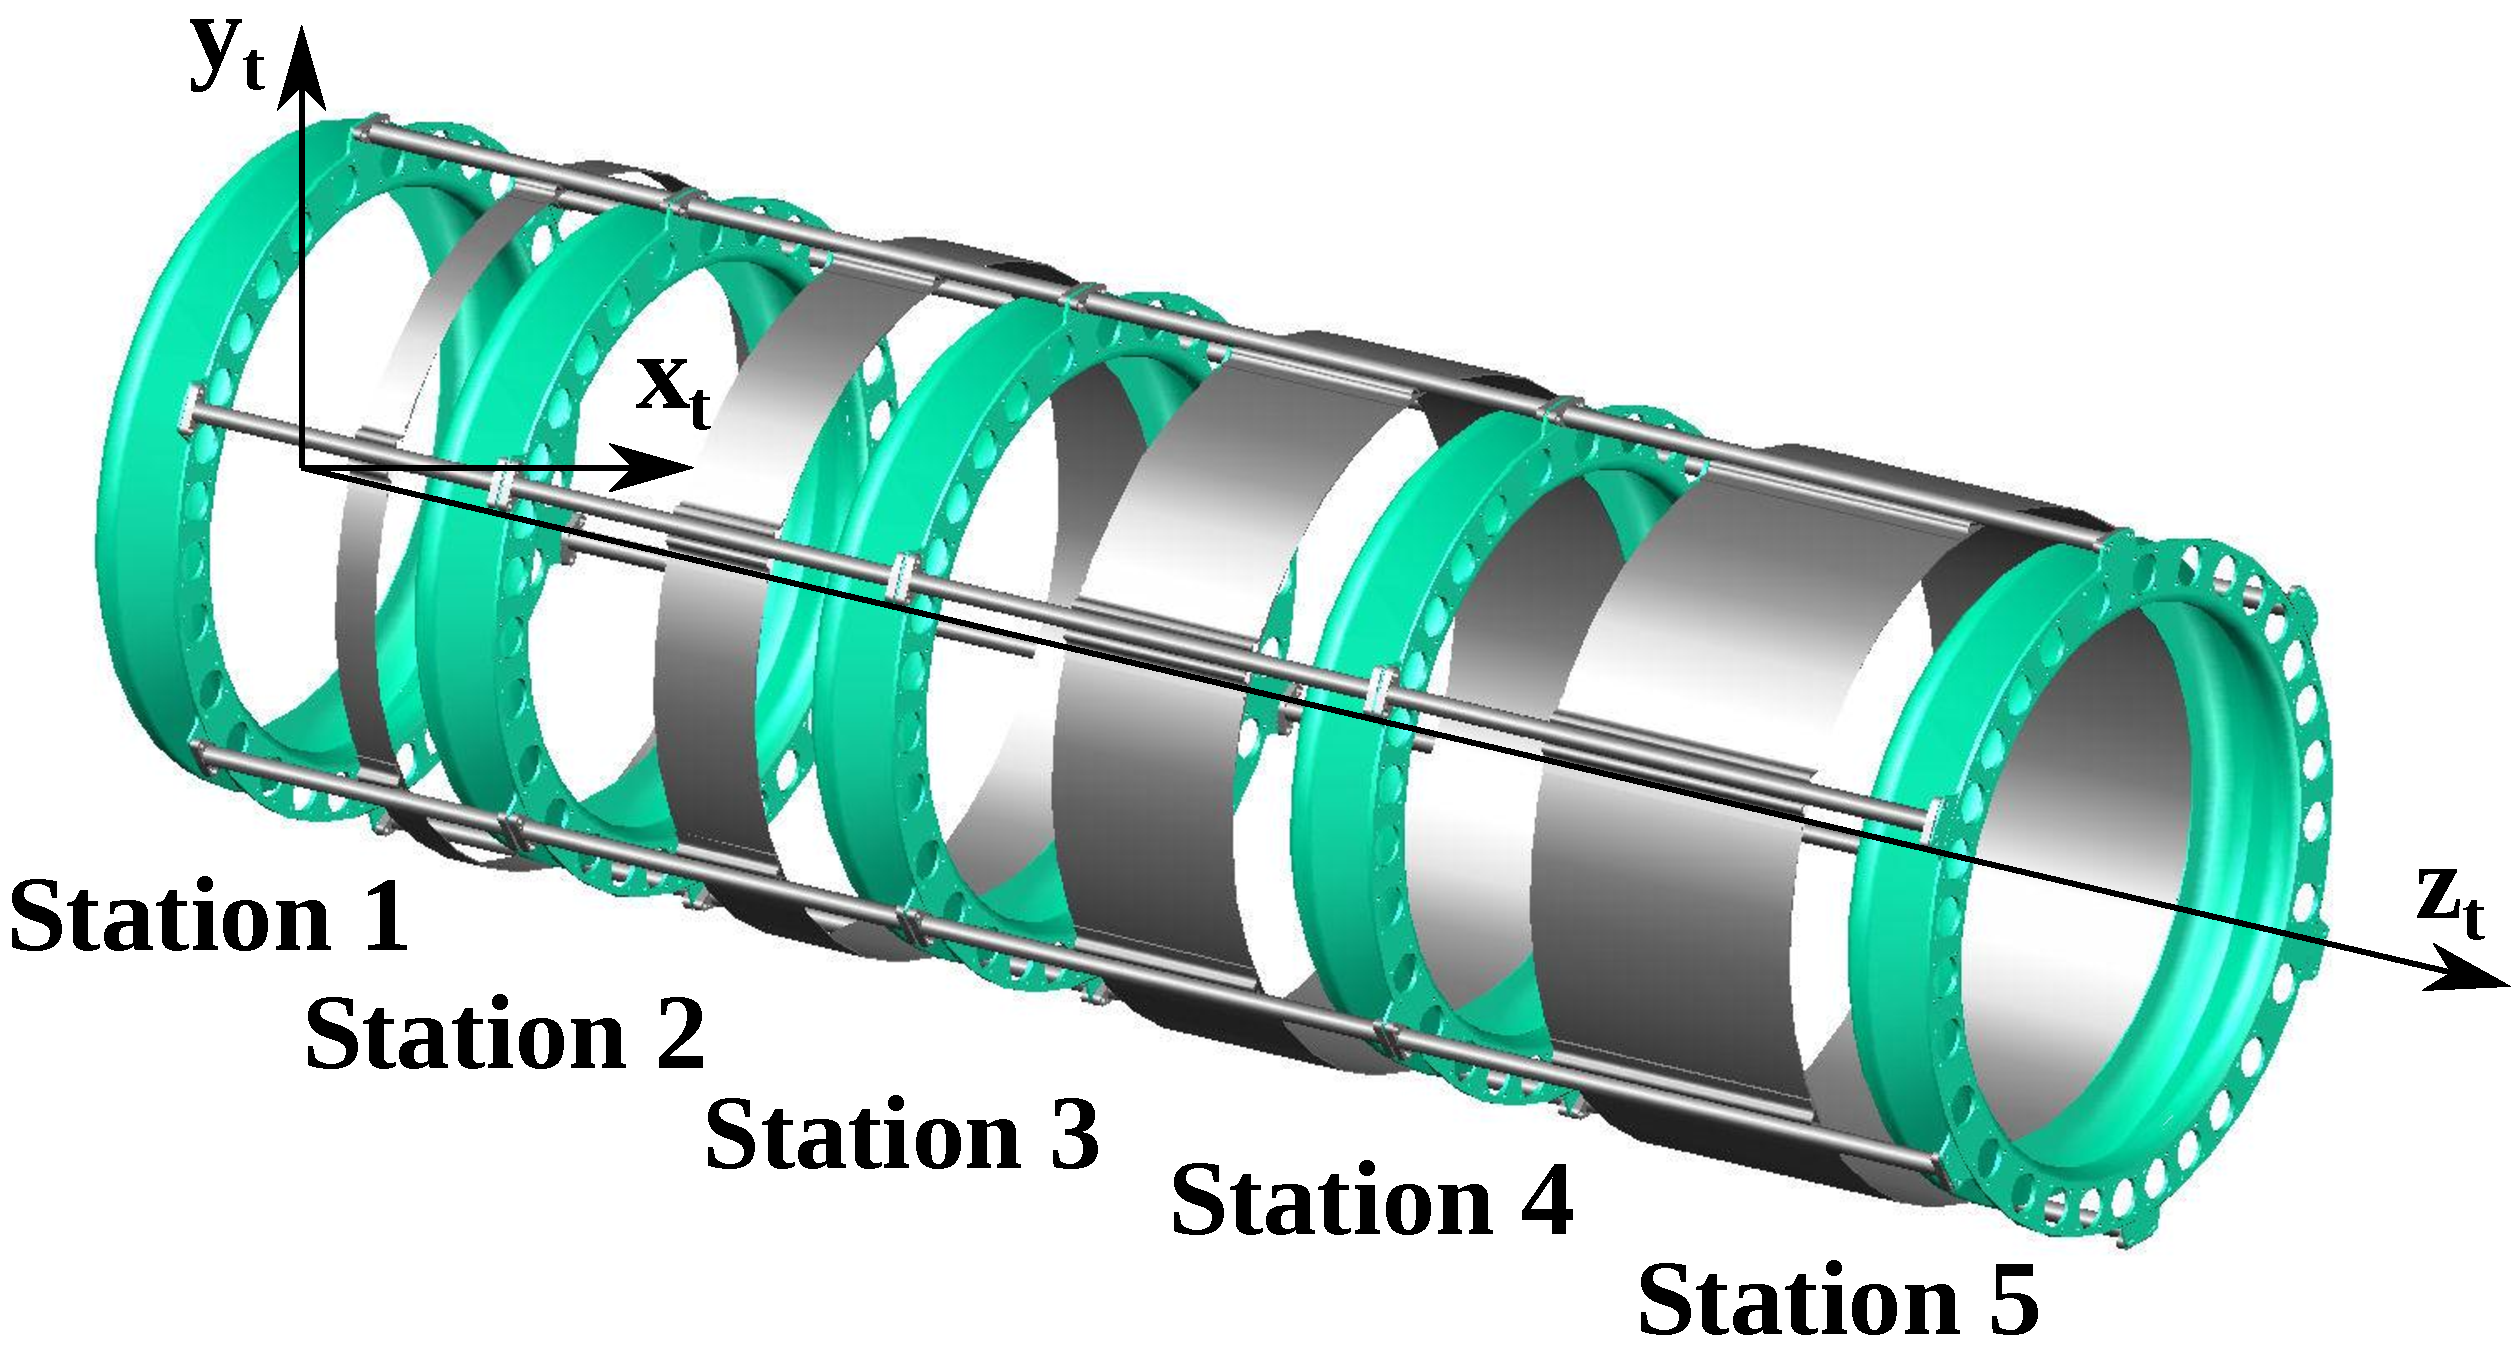
\includegraphics[width=0.5\linewidth]{01-MICE/TrackerFrame.pdf} \hspace{2pc}%
    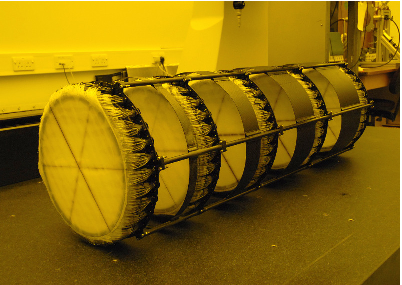
\includegraphics[width=0.35\linewidth]{01-MICE/TrackerPhoto.pdf}
    \caption{\label{fig:Trackers} Left: A schematic of the tracker carbon fibre frame, showing the detector station positions.  The fibre planes are glued on to the upstream edge (smaller $z_t$ position) of the carbon fibre station frames (shown in green). Right: A photograph of a tracker. The orange tint is due to the special lighting needed to protect the fibres. The intersecting lines visible on the station faces indicates the direction of the fibres in each plane.}
  \end{figure}

  Each station is formed of three planes of 350~$\mu$m scintillating fibres, orientated at 120 degrees to each other, attached to a sheet of mylar plastic. The fibres in each plane are arranged in a doublet-layer structure in order to give 100$\%$ coverage of the plane area as illustrated in figure~\ref{fig:DoubletLayer}. A mylar sheet glued to the doublet layer provides mechanical stability. The fibres are collected into groups of seven for readout, each group forming a single channel, as illustrated in figure~\ref{fig:DoubletLayer}b. The planes, also known as views, are labelled $U$, $V$ and $W$. Plane $U$ is attached to the station frame directly, plane $W$ on to plane $U$, and plane $V$ on to plane $W$. The fibre plane orientations are illustrated in figure~\ref{fig:FibrePlaneOrientation}. Each station is oriented such that the fibres in the U plane are vertical. The fibres produce scintillation light when ionising radiation passes through them. Clear-fibre light guides transport the scintillation light to visible light photon counters (VLPCs) in a cryostat for readout (see~\cite{MiceTrackers} for details).

  \begin{figure}[tbh]
    \begin{center}
      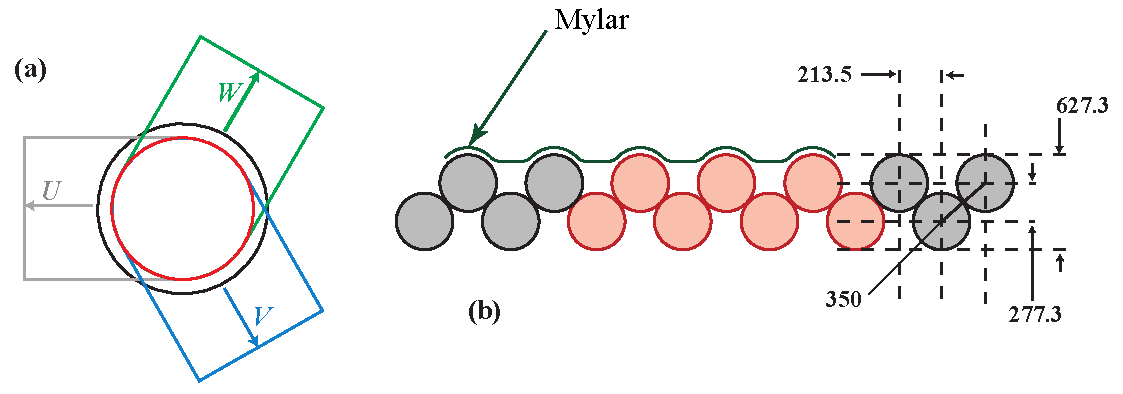
\includegraphics[width=0.85\textwidth]{01-MICE/doublet-layer.pdf}
      \caption{\label{fig:DoubletLayer}(a) Arrangement of the doublet layers in the scintillating-fibre  stations. The outer circle shows the solenoid bore while the inner circle shows the limit of the active area of the tracker. The arrows indicate the direction that the individual 350\,$\mu$m fibres run. (b) Detail of the arrangement of the scintillating fibres in a doublet layer. The fibre spacing and the fibre pitch are indicated on the right-hand end of the figure in \,$\mu$m. The pattern of seven fibres ganged for readout as a single channel, via a single clear-fibre light-guide, is shown in red. The sheet of mylar plastic glued to the doublet layer is indicated. }
    \end{center}
  \end{figure}

  \begin{figure}[tbh]
    \centering
    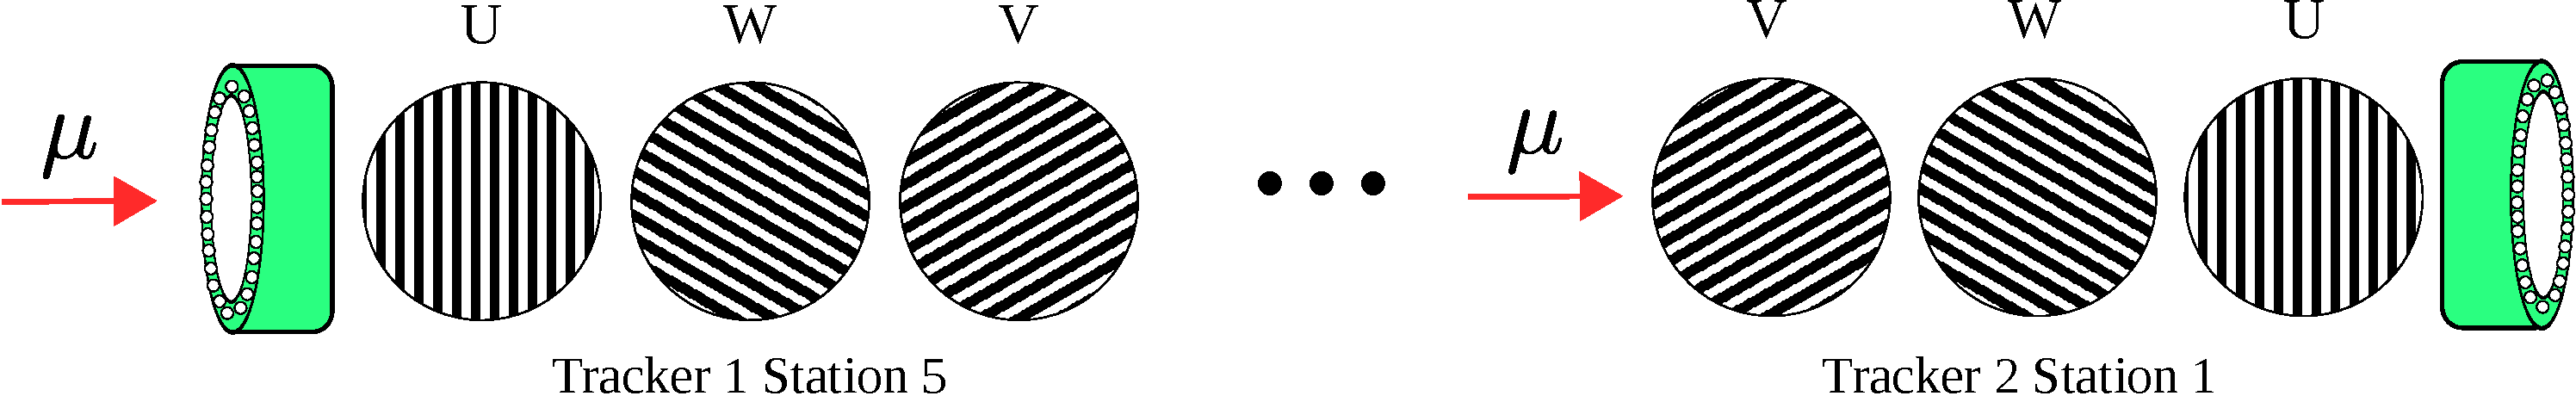
\includegraphics[width=0.95\linewidth]{01-MICE/FibrePlaneOrientation.pdf} \hspace{2pc}%
    \caption{\label{fig:FibrePlaneOrientation} The orientation of the fibres in each plane, as seen be the incoming beam, for both trackers. The green object is station frame. If TKU was rotated by $180^\circ$ around the centre of the cooling channel, it would be coincident  TKD.}
  \end{figure}